%********************************************************************
% Experiments
%*******************************************************
% If problems with the headers: get headings in appendix etc. right
%\markboth{\spacedlowsmallcaps{Appendix}}{\spacedlowsmallcaps{Appendix}}
\chapter{Experiments}\label{ch:experiments}
\glsresetall % Resets all acronyms to not used
In this chapter, it is described how and what experiments were conducted. It is described how NEAT-TCP NNs are evaluated and how the congestion window is changed as well as which fitness functions and which parameters for the NEAT evolution were used.

\section{Experiment Setup}\label{sec:expsetup}
All experiments were conducted with an Intel Core i7-4790k not overclocked and running Ubuntu 16.04 LTS. Because ns-3 can not be used in parallel, as mentioned in \autoref{subsec:parallelisation}, all experiments are running on a single thread. \\
For all experiments a maximum of 100 epochs of evolution is used. We only use 100 epochs because after 100 epochs there were no significant improvements observed. \\ The network is simulated for 40 seconds. The reason is, that with a low simulation time, the simulation does need less time to be calculated. And because 50,000 simulations need to be calculated in the worst case, the simulation time is set low. In future works, with more time on hand, it should be set higher or different network configurations per evaluation should be taken into consideration. This is discussed further in \autoref{sec:futureWork}.


\subsection{NEAT-TCP Configuration Combinations in Experiments}\label{subsec:configurations}
There are seemingly endless ways how NEAT-TCP can be configured. The activation function and the time at which the NN is evaluated can be freely set, but only one activation function can be used at a time, because NEAT has no support for multiple activation functions within the same neural network. We use two different activation functions, three different ways how the NN is evaluated and two different points of time at which the NN is evaluated, to a total of twelve experiments.\\
\textbf{Activation Functions:} 
\begin{equation}\label{eq:sigmoid}
\phi_1(x)=\left\{\begin{matrix}
1 & , x> 0\\ 
 0 & , \text{else}
\end{matrix}\right.
\end{equation}
\begin{equation}\label{eq:identity}
\phi_2(x)=x
\end{equation}
As for \autoref{eq:sigmoid} a rectifier function is used. A node is activated if the activation sum is positive, otherwise it is not activated. This function is used for decision making, where it can decide between two decisions. \\
As for \autoref{eq:identity} an identity function is used. This means that the output can range continuously in value. This function is used for a higher variety of decisions, for the number of segments that are added or subtracted to the congestion window, or set to the new congestion window, like in these experiments.\\\\
\textbf{Congestion Window Formulas}\\
There are endless possibilities for the congestion window formula or how the NN is incorporated.
In general the congestion window formula has to be attuned to the used activation function.
For example, if $\phi_1$ is used, then it would not make sense to add the result to the congestion window as it would take at least 536 evaluations until more could be sent.
The following equations describe how the congestion window is manipulated.
\begin{equation}\label{eq:add}
\text{cwnd1: \quad} \text{cwnd} = \text{cwnd} + \text{out} * \text{MSS}	
\end{equation}

\begin{equation}\label{eq:direct}
\text{cwnd2: \quad} \text{cwnd} = \text{out} * \text{MSS}	
\end{equation}

\begin{equation}\label{eq:sigAdd}
\text{cwnd3: \quad} \text{cwnd} = \left\{\begin{matrix}
\text{cwnd} + \text{MSS}, & \text{out} > 0\\ 
\text{cwnd} - \text{MSS}, & \text{else}
\end{matrix}\right.
\end{equation}
Where \textit{out} is the value that is received from the NN and \textit{MSS} is the maximum segment size.\\\\

\textbf{NN Evaluation Times}\\
There are endless possibilities, at what time the NN could be evaluated. It could be evaluated periodically, i.e. every 10 ms. Or it can be evaluated depending on events happening in the socket, while a combination of timer and event-based evaluation is also possible. The possibilities are sheer endless. 
We use two different event-based time points where the NN is evaluated:
\begin{itemize}
	\item{PktAcked: The NN is evaluated every time a packet is acknowledged.}
	\item{Increase Window: The NN is evaluated every time the function IncreaseWindow is called in \texttt{tcp-socket-base}. This is the same time where TCP New Reno would be called for its slow start or AIMD.}
\end{itemize}
These time points are the ones that normally call the associated congestion control algorithm. For example, \texttt{Increase Window} is implemented by TCP New Reno and provides its functions of slow start and congestion avoidance there. 

\textbf{List of Experiments:}
All of the following experiments have been conducted once, because of time constraints. Each experiment conducts up to 50,000 simulations.
\begin{itemize}
	\item{Experiment1: PktAcked, $\phi_1$, cwnd3, $\rho_1$}
	\item{Experiment2: PktAcked, $\phi_2$, cwnd1, $\rho_1$}
	\item{Experiment3: PktAcked, $\phi_2$, cwnd2, $\rho_1$}
	\item{Experiment4: Increase Window, $\phi_1$, cwnd3, $\rho_1$}
	\item{Experiment5: Increase Window, $\phi_2$, cwnd1, $\rho_1$}
	\item{Experiment6: Increase Window, $\phi_2$, cwnd2, $\rho_1$}
	\item{Experiment7: PktAcked, $\phi_1$, cwnd3, $\rho_2$}
	\item{Experiment8: PktAcked, $\phi_2$, cwnd1, $\rho_2$}
	\item{Experiment9: PktAcked, $\phi_2$, cwnd2, $\rho_2$}
	\item{Experiment10: Increase Window, $\phi_1$, cwnd3, $\rho_2$}
	\item{Experiment11: Increase Window, $\phi_2$, cwnd1, $\rho_2$}
	\item{Experiment12: Increase Window, $\phi_2$, cwnd2, $\rho_2$}
\end{itemize}

\subsection{NEAT Parameter File}\label{subsec:neatparameter}
For the NEAT parameter file \texttt{p2nv.ne} is used. This file is provided with NEAT and is intented to solve the non-Markovian double pole balancing without velocity information. Further discussion on why we used this specific parameter file can be found in \autoref{sec:congVSbalancing}. The significant parameters are:
\begin{itemize}
	\item{Weight Mutation Power: 1.8. Describes how much the link weight is changed in the \textit{Link Weight Mutation}.}
	\item{Recurrent Probability: 5\%. The probability a newly created link is recurrent, where the link is resolving and going into the same node. This implements memory, because the result of the recurrent link has influence on the next evaluation of the NN. }
	\item{Mutate Link Probability: 80\%. Probability a link weight is mutated.}
	\item{Toggle Enable Probability: 10\%. The probability a link is disabled or enabled.}
	\item{Add Node Probabilty: 1\%. The probability a new node is added to the NN.}
	\item{Add Link Probability: 30\%. The probability a link is added to the NN.}
	\item{Population Size: 500 organisms.}
	\item{Dropoff Age: 15. A NN is only able to survive for a maximum of 15 epochs.}
	
\end{itemize}
All parameters, besides \textit{Population Size} and \textit{Dropoff Age} are used in the mutation step, \autoref{fig:neatIteration}. The \textit{Population Size} is an initialisation factor that is maintained through the whole evolution and the \textit{Dropoff Age} is one of the factors of the elimination step.


\subsection{Network Specification}\label{subsec:networkspec}
\begin{figure}[h]
	\centering
	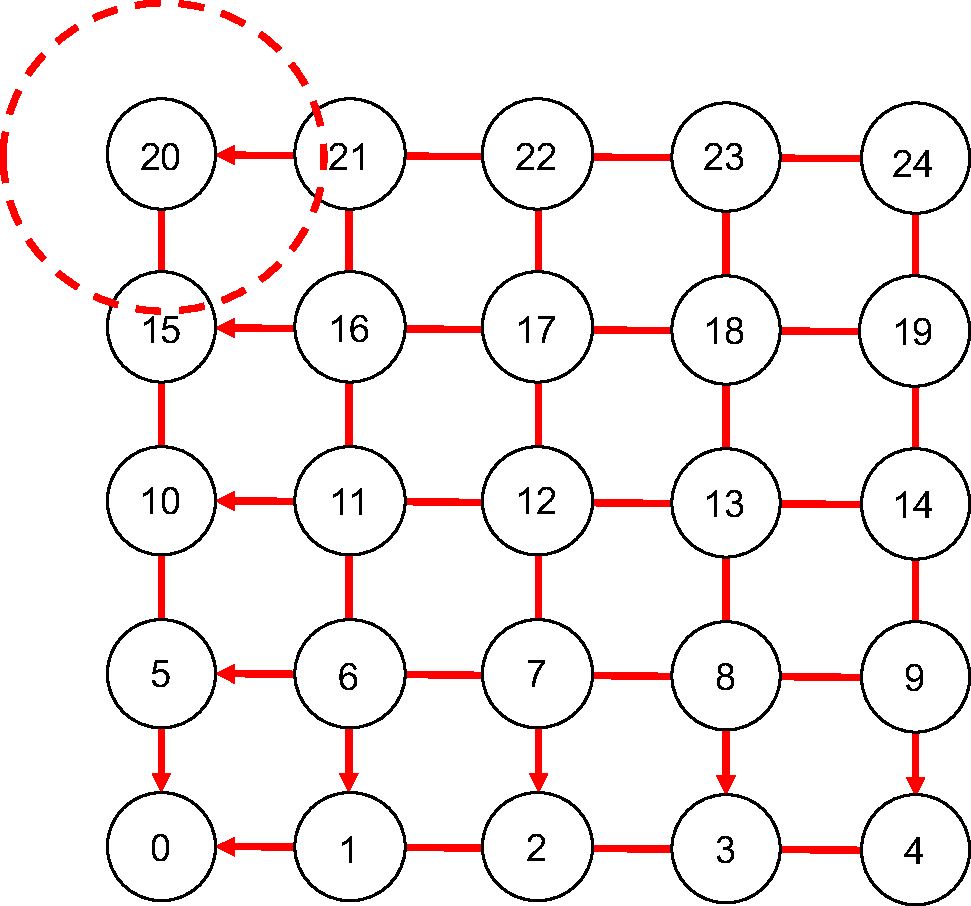
\includegraphics[scale=0.45]{networkTopology}
	\caption{Wireless grid network topology}
	\label{fig:networkTop}
\end{figure}
ns-3 has an example of a simple ad-hoc grid network, defined in \texttt{examples/wireless/wifi-simple-adhoc-grid}. This network specification is built on this example. A 2-D grid is built with 25 nodes in a 5x5 manner. All nodes can only reach their horizontal and vertical neighbours, but not their diagonal neighbours. So the maximum hop count is 8, from the node on the bottom left to the one on the top right. The physical layer is taken from the example with no changes. RTS/CTS is enabled for all packets that are above 100 bytes, that means the routing does not use it, which speeds up the simulation. The receiver and sender buffer size is set to 26800 bytes which is about 50 packets. There are 10 TCP flows sending from one side to the opposite in this grid. A visualisation can be found in \autoref{fig:networkTop}. All flows start at the same time and all try to send with a data rate of 1MBps. The radio is only capable of sending this much, so congestion is guaranteed.

\subsection{Fitness Functions}\label{subsec:fitnessfunc}
Two different fitness function are used:
\begin{equation}\label{eq:fitness1}
\rho_1 = \frac{\tau_a^\sigma}{\tau_t^\sigma}*\mathcal{J} 
\end{equation}
\begin{equation}\label{eq:fitness2}
\rho_2 = \tau_a^\sigma
\end{equation}
\begin{figure}\label{fig:jain}
\[ \ \qquad \qquad \quad \mathcal{J} (x_1, x_2, \dots, x_n) = \frac{( \sum_{i=1}^n x_i )^2}{n \cdot \sum_{i=1}^n {x_i}^2}\]
\caption{Jain`s fairness index}
\end{figure}
Where $\tau_a^\sigma$ is the achieved total throughput, $\tau_t^\sigma$ is the target total throughput and $\mathcal{J}$ is the Jain`s fairness index.
For \autoref{eq:fitness1} the achieved total throughput (sum of throughputs of all flows in the network) is normalised over the target total throughput and multiplied by the achieved fairness. The fairness, Figure 14, is calculated with the received bytes of the different flows. This leads to 1 if the target total throughput is achieved with perfect fairness. Because this is unlikely to be achieved thence a certain throughput, the target fitness in the evaluation of \texttt{experiments} should be chosen below 1, which is why we use a target fitness of 0.9.\\
For \autoref{eq:fitness2} only the achieved total throughput is considered. This neglects fairness, which means that the resulting NNs are prone to be unfair.


%********************************************************************
% Evaluation
%*******************************************************
% If problems with the headers: get headings in appendix etc. right
%\markboth{\spacedlowsmallcaps{Appendix}}{\spacedlowsmallcaps{Appendix}}
\chapter{Evaluation}\label{ch:evaluation}
\glsresetall % Resets all acronyms to not used

\section{Results of the Conducted Experiments}\label{sec:expResults}
\autoref{tab:evoResults} shows the results of the experiments described in \autoref{subsec:configurations}. The following section is divided into two parts differing by the used fitness function. The performance of the best NNs of experiments 1-6 and 7-12 is visualised in \autoref{sec:resCompare}.
\begin{table}[h]
\centering
\caption{NEAT-TCP experiments results}
\begin{tabular}{|l|l|l|}\hline
Experiment & Highest Fitness Achieved & Epoch of Best Performing NN  \\ \hline
    1       &              0.901888            &             10          \\ \hline
    2      &                0.641739          &               23         \\ \hline
    3      &                 0.683554         &               86        \\ \hline
    4       &               0.832359           &           71           \\ \hline
    5      &                  0.721011        &              79          \\ \hline
    6      &                0.740281          &              27         \\ \hline
    7       &            526.596              &              78         \\ \hline
    8      &              366.877            &              48          \\ \hline
    9      &             369.302             &            75           \\ \hline
  10       &              524.958            &              59         \\ \hline
  11      &               423.408           &            41            \\ \hline
   12      &             427.743             &           85            \\ \hline
\end{tabular}

\label{tab:evoResults}
\end{table}
\subsection{Results for Fitness: $\rho_1$}\label{subsec:resultsFitness1}
 For $\rho_1$ (experiments 1-6) with a target throughput of 400 kbits, the best performing NNs have been evolved by experiment 1 and 4, which both use $\phi_1$ as their activation function. This could indicate, that this setup of $\phi_1$ and cwnd3 is superior to the other configurations. But all of these experiments were conducted only once and only with one parameter file, due to time constraints. It could be the case that the used parameter file privileges $\phi_1$ and not $\phi_2$. The decisive parameter could be \textit{Weight Mutation Power}.  Since $\phi_2$ is an identity function and the output is needed to be a relatively high number, in relation to $\phi_1$, it could be the case that the weights are not mutated sufficiently to reach these numbers. 

 
\subsection{Results for Fitness: $\rho_2$}\label{subsec:resultsFitness2}
As for the experiments with $\rho_2$, the same behaviour can be observed. The two best performing NNs again have the setup of $\phi_2$ and cwnd3, with a slight, but negligible edge in favour of the evaluation at PktAck. So, the assumption that \texttt{p2nv.ne} favours this setup, does still hold up here and is discussed in detail in \autoref{subsec:diffNEATpar}.
  
\section{Evaluation Setup}\label{sec:evalSetup}
We evaluate the different generated NEAT-TCP neural networks in comparison with iTCP and TCP New Reno. For every grid 100 simulations are conducted to get statistical significance. Measures are gathered every five seconds after 40 seconds of simulation time, there the measures have more meaning, after the routing has finished, flows are connected and should have balanced out. We average all 100 values for every measure for every five seconds to overcome overplotting and get an idea of how the different TCP flavours behave in general. Then we present a snapshot of the final state at 300 seconds simulation time with all values collected. For these snapshots box and whisker charts are used, that show the distribution of data in quartiles. The mean is highlighted and the whiskers indicate variability outside the upper and lower quartiles. All dots in these charts are outliers.

\section{Evaluation of Various Performance Metrics}\label{sec:resCompare}
In this section, TCP New Reno, iTCP in different configurations and the best NEAT-TCP NNs of experiments 1-6 and experiments 7-12 are compared to each other in relation to total network throughput, fairness, mean end-to-end delay and packet loss.\\
The best NEAT-TCP evolved with fitness $\rho_1$ is further called \textit{NEAT-TCP1} and NEAT-TCP evolved with fitness $\rho_2$ is further called \textit{NEAT-TCP2}.\\
For iTCP we evaluate the in \autoref{sec:itcpimpl} defined configurations. We further call iTCP: \textit{iTCP-bytes} for the byte-fed iTCP with a maximum of 2680 bytes (5 segments) and \textit{iTCP-seg} for the segments-fed iTCP with a maximum of 5 segments (2680 bytes). It is expected that \textit{iTCP-seg} performs better, because the activation functions are attuned to the number of segments. \\


\subsection{Throughput}\label{subsec:throughput}
In \autoref{fig:plotThroughput} it can be seen, that \textit{iTCP-bytes} takes the longest time to converge at about 200 s simulation time, with \textit{New Reno} being the second slowest in terms of convergence with about 150 s simulation time. In comparison, \textit{iTCP-seg}, \textit{NEAT-TCP1} and \textit{NEAT-TCP2} are already balanced out at 40 s simulation time and only increasing slowly, which may be because of how the total throughput is calculated. \\
It can be seen that a simulation time of 40 s in the evolution of NEAT-TCP is sufficient and projects its behaviour for longer simulations. It may also favour the evolved NNs, because with less time to reach certain measures, these measures have to be reached faster, resulting in a more consistent behaviour.

\begin{figure}[h]
	\centering
	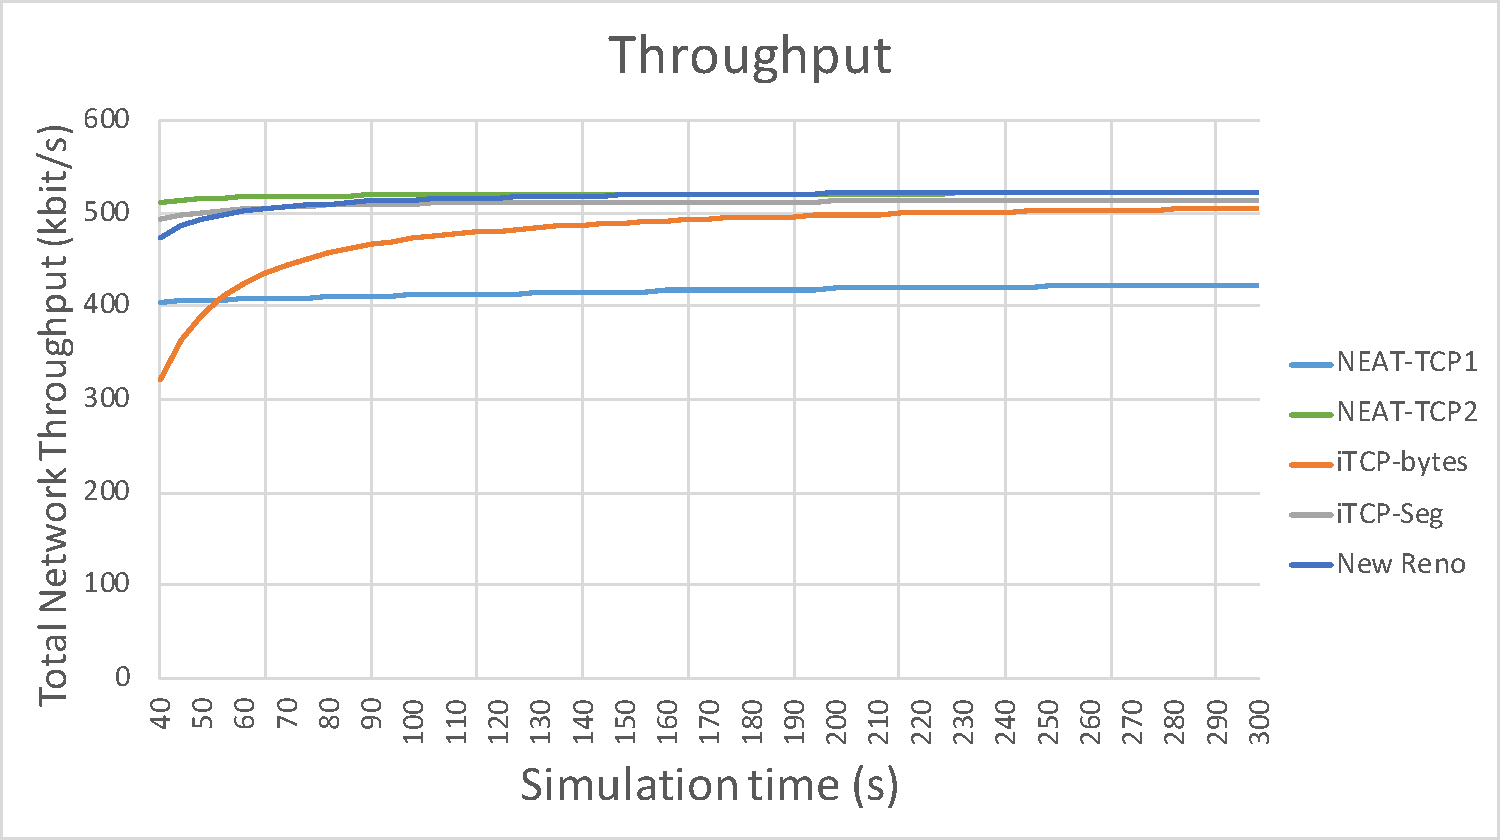
\includegraphics[width=1\textwidth]{plotThroughput}
	\caption{Throughput over simulation time}
	\label{fig:plotThroughput}
\end{figure}
In \autoref{fig:boxThroughput} the snapshot at 300 s is shown. It can be seen that all flavours, besides \textit{NEAT-TCP1}, have comparable throughput with little variance, whereas \textit{NEAT-TCP1} has less throughput than the others with a higher variance. 
\begin{figure}[!h]
	\centering
	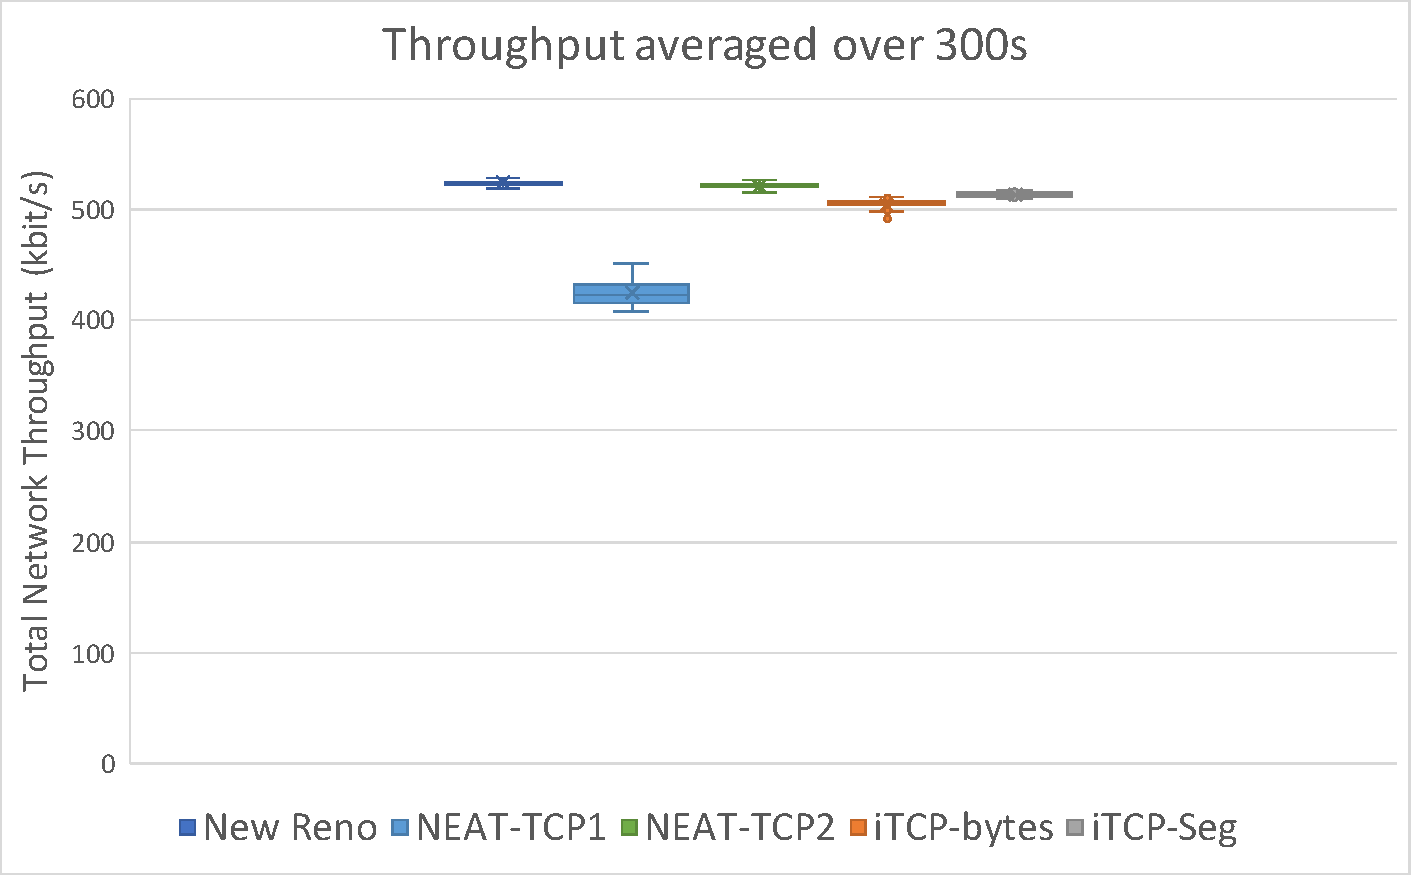
\includegraphics[width=1\textwidth]{boxThroughput}
	\caption{Throughput at 300 s simulation time}
	\label{fig:boxThroughput}
\end{figure}

\subsection{Fairness}\label{subsec:fairness}
Fairness is the Jain`s fairness index, Figure 14, with the bytes received at each sink node. 
The fairness is expected to decrease over time, because it is calculated with the received bytes.
 As more bytes are received, the differences in bytes received at each sink node increases if there are various different throughputs in the network.
\begin{figure}[h]
	\centering
	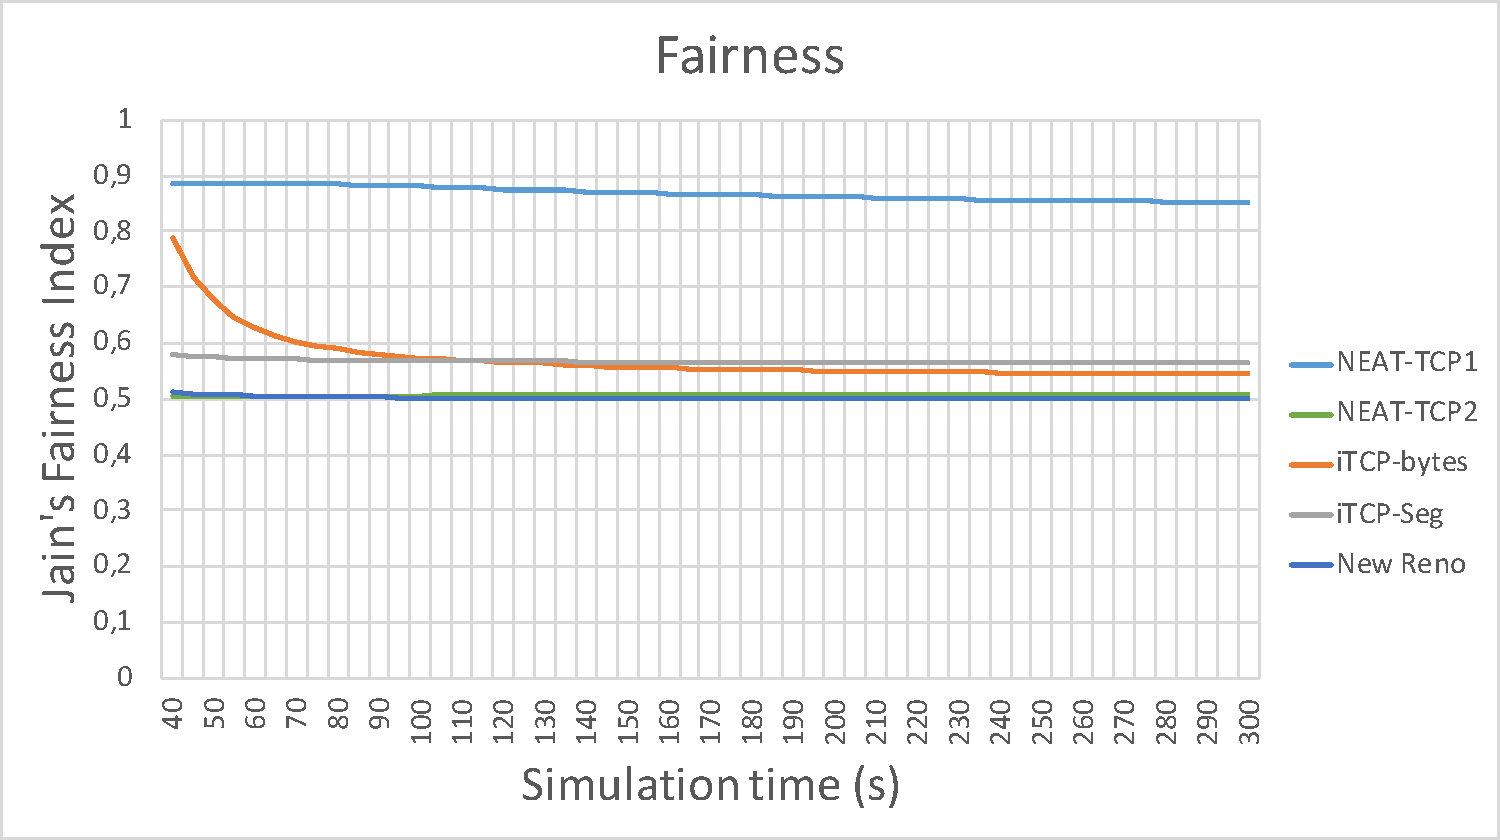
\includegraphics[width=1\textwidth]{plotFairness}
	\caption{Fairness over simulation time}
	\label{fig:plotFairness}
\end{figure}
In \autoref{fig:plotFairness} it can be seen that the fairness of \textit{NEAT-TCP1} is slowly decreasing, as prior mentioned, because of how the fairness is calculated.
\textit{iTCP-bytes} on the other hand has a strong decrease in fairness in the early stages. This indicates that flows are cut out as the simulation progresses. Also it can be seen, that fairness behaves inverse proportional to throughput for \textit{iTCP-bytes}. As throughput increases, fairness decreases. So as flows are gaining higher throughput, some flows are overpowered and finally cut out. 
As for \textit{iTCP-seg}, \textit{NEAT-TCP2} and \textit{New Reno} the fairness is constant. It is observed that for every flavour, besides \textit{NEAT-TCP1}, at least two flows are cut out within the progression of the simulation.
\begin{figure}[h]
	\centering
	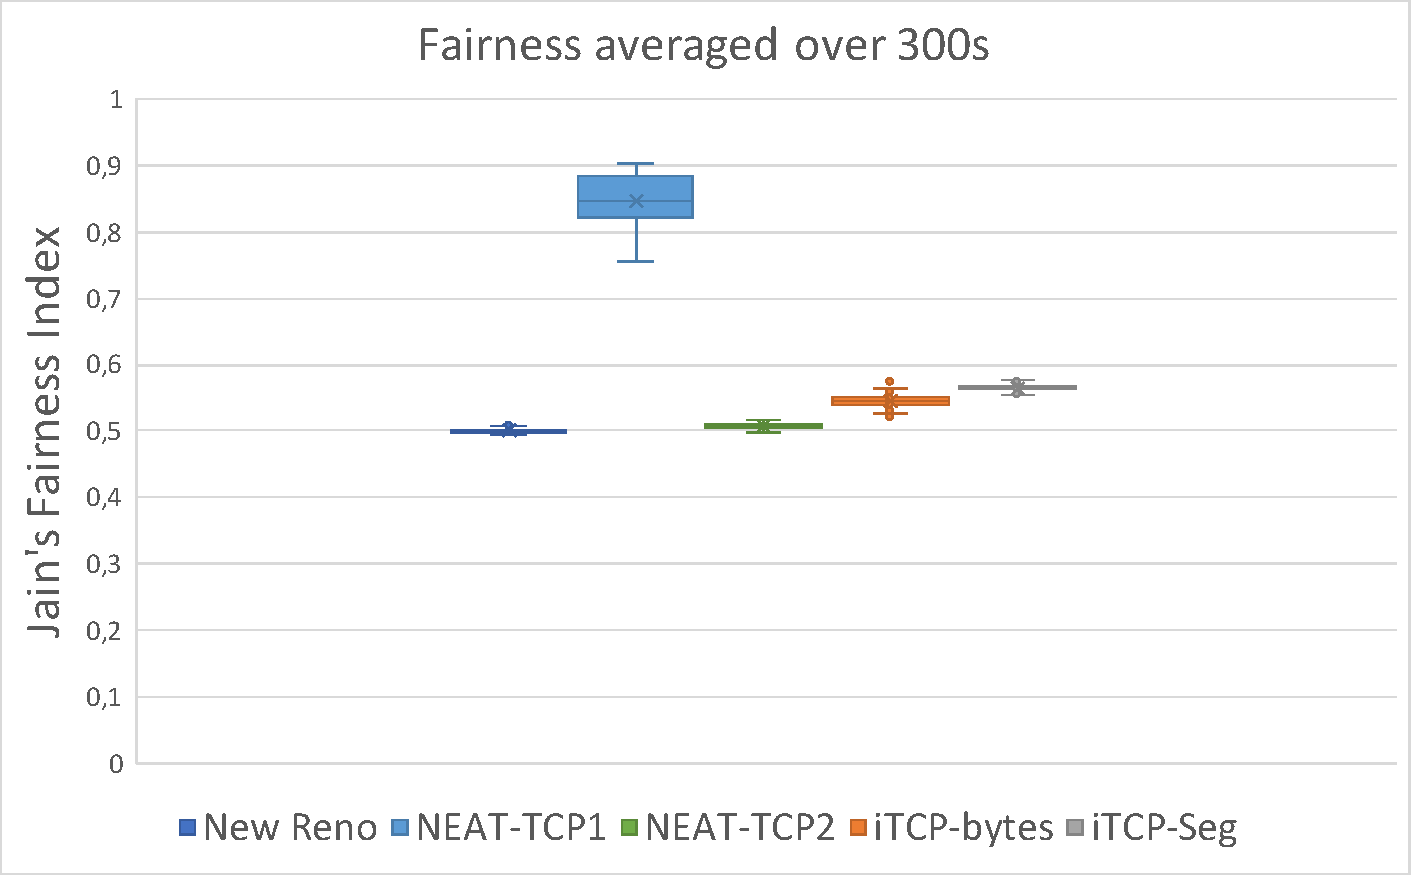
\includegraphics[width=1\textwidth]{boxFairness}
	\caption{Fairness at 300 s simulation time}
	\label{fig:boxFairness}
\end{figure}
In \autoref{fig:boxFairness} the snapshot at 300 s is shown. Again, as with throughput, \textit{NEAT-TCP1} has the most variance, but has the highest fairness. 
\textit{New Reno} and \textit{NEAT-TCP2} both have comparable fairness, but both iTCP flavours have better fairness than them with \textit{iTCP-seg} being the one with the best fairness besides \textit{NEAT-TCP1}.
\newpage


\subsection{Mean End-to-End Delay}\label{subsec:meanDelay}
Mean end-to-end delay is calculated by taking the end-to-end delay sum and dividing it by the number of sent packets. This includes lost packets, so timeouts are considered. 
\begin{figure}[h]
	\centering
	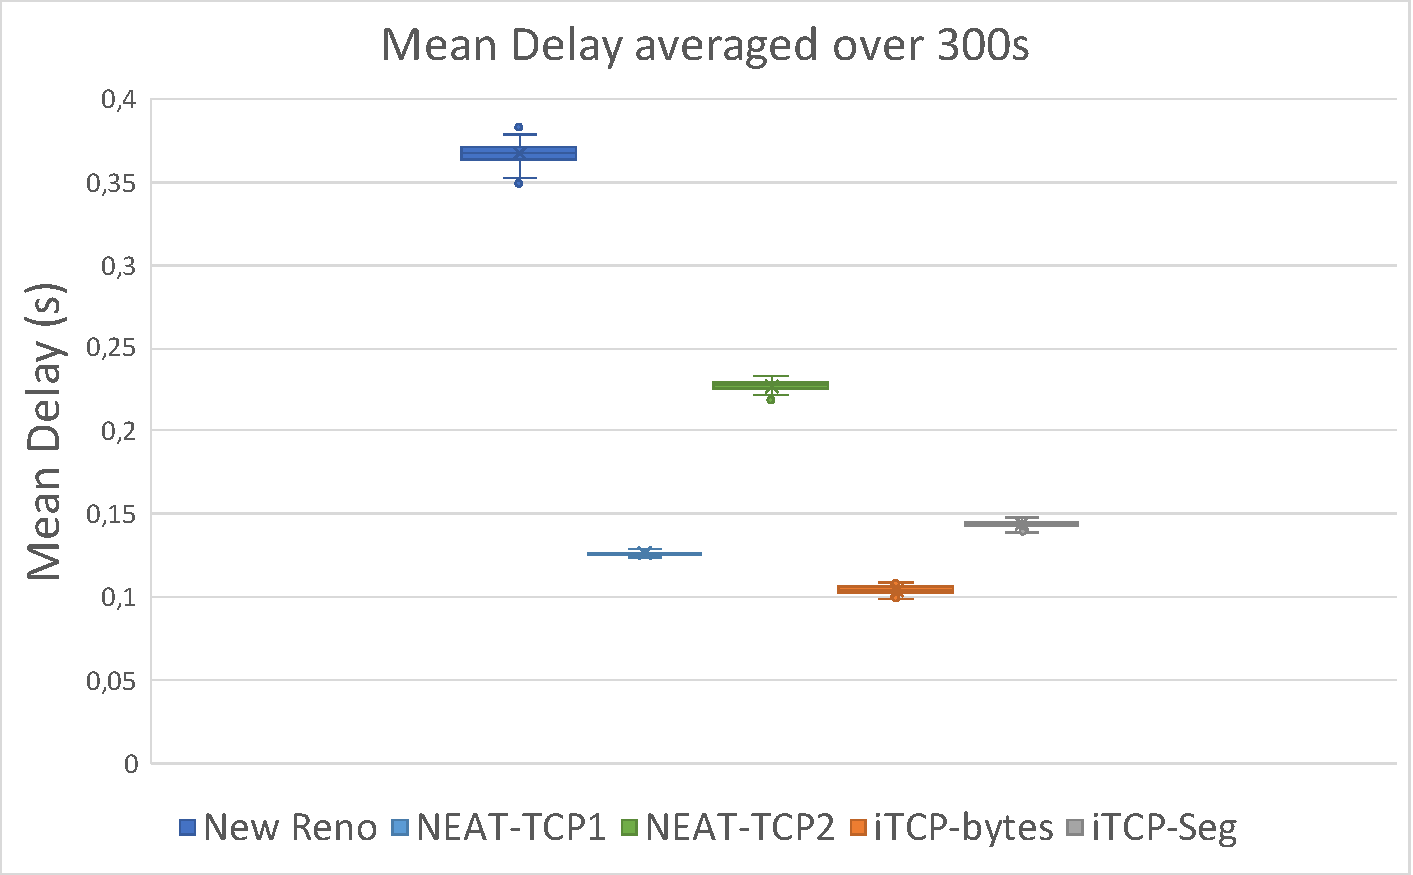
\includegraphics[width=1\textwidth]{boxDelay}
	\caption{Mean delay at 300 s simulation time}
	\label{fig:boxDelay}
\end{figure}
In \autoref{fig:boxDelay}, it can be seen that \textit{New Reno} has the highest delay overall, followed by \textit{NEAT-TCP2}. \textit{iTCP-bytes} has the lowest mean end-to-end delay overall. \textit{NEAT-TCP1} has a slightly higher mean end-to-end delay than \textit{iTCP-bytes}, but lower than \textit{iTCP-seg}.
\subsection{Packet Loss}\label{subsec:lostPacktes}
Packet loss is calculated by dividing the number of lost packets by the number of transmitted packets. 

\begin{figure}[h]
	\centering
	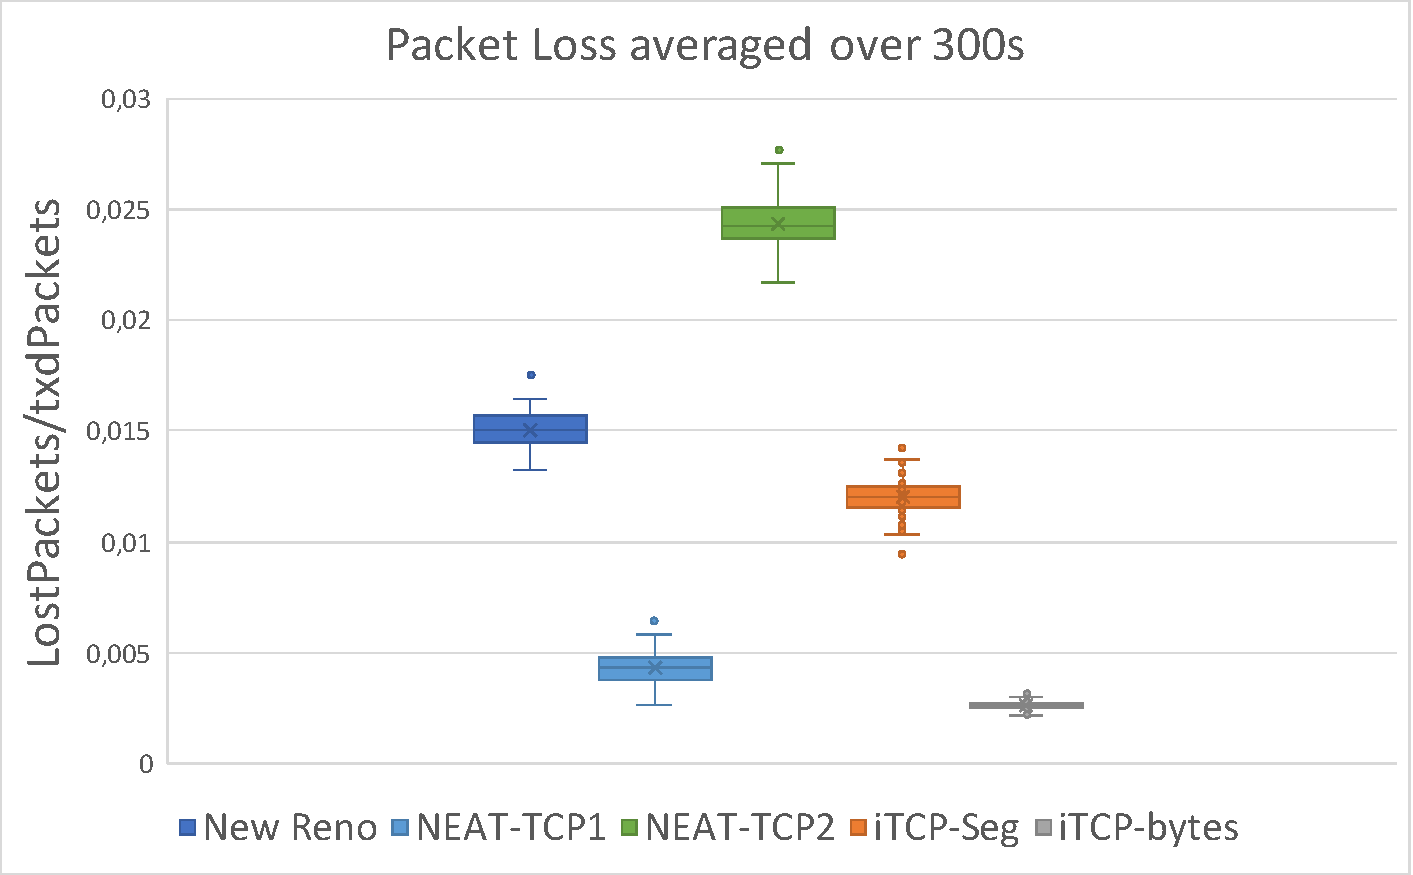
\includegraphics[width=1\textwidth]{boxPktLoss}
	\caption{Packet loss at 300 s simulation time}
	\label{fig:boxPktLoss}
\end{figure}
In \autoref{fig:boxPktLoss} it can be seen that \textit{iTCP-bytes} loses the least amount of packets, followed by \textit{NEAT-TCP1}. Both of them lose below 1\% of the transmitted packets. \textit{New Reno} and \textit{iTCP-seg} populate the midfield by losing less than 2\% of the transmitted packets. And \textit{NEAT-TCP2} loses the most packets among the evaluated flavours.

\subsection{Performance in Different Network Configurations}\label{subsec:perf3x3}
We tested the different congestion control algorithms in other networks, 3x3 and 6x6, but the rest of the network configuration is the same as in \autoref{subsec:networkspec}. We did this in order to see how NEAT-TCP behaves in other environments it was not evolved for. In \autoref{tab:3x3} and \autoref{tab:6x6} the performance at 300 seconds simulation time of \textit{NEAT-TCP1, NEAT-TCP2, iTCP-bytes} and \textit{iTCP-seg} is printed with New Reno as a baseline.

% Table generated by Excel2LaTeX from sheet 'Sheet9'
\begin{table}[htbp]
  \centering
  \caption{3x3 results at 300 seconds simulation time in relation to New Reno}
    \begin{tabular}{|l|r|r|r|r|}\hline
    3x3   & \multicolumn{1}{l|}{Throughput} & \multicolumn{1}{l|}{Fairness} & \multicolumn{1}{l|}{Delay} & \multicolumn{1}{l|}{Packet loss} \\\hline
    New Reno & 420.591 kbit/s & 0.562453 & 0.19120473 s & 2.32 \% \\\hline
    NEAT-TCP1 & -18.10\% & +57.73\% & -55.40\% & -41.00\% \\\hline
    NEAT-TCP2 & -4.42\% & +14.12\% & -9.57\% & +28.50\% \\\hline
    iTCP-seg & -7.04\% & +22.52\% & -45.59\% & -17.72\% \\\hline
    iTCP-bytes & -6.12\% & -9.42\% & -74.55\% & -64.01\% \\\hline
    \end{tabular}%
  \label{tab:3x3}%
\end{table}%
It can be seen in \autoref{tab:3x3} that \textit{NEAT-TCP1} behaves the same in relation to \textit{New Reno} in 3x3 as in 5x5, \autoref{tab:resultsCompare}. It still lowers the throughput, mean end-to-end delay and packet loss, while increasing fairness significantly. As for \textit{NEAT-TCP2} a different behaviour can be observed. It now increases fairness while having slightly less throughput. 
As for \textit{iTCP-seg} and \textit{iTCP-bytes} similar behaviour can be observed, but \textit{iTCP-bytes} now decreases fairness by about the percentage as it increases in 5x5, in relation to \textit{New Reno}.
% Table generated by Excel2LaTeX from sheet 'Sheet9'
\begin{table}[htbp]
  \centering
  \caption{6x6 results at 300 seconds simulation time in relation to New Reno}
    \begin{tabular}{|l|r|r|r|r|}\hline
    6x6   & \multicolumn{1}{l|}{Throughput} & \multicolumn{1}{l|}{Fairness} & \multicolumn{1}{l|}{Delay} & \multicolumn{1}{l|}{Packet loss} \\\hline
    New Reno & 1564.26 kbit/s & 0.457674 & 0.22629042 s & 0.86\% \\\hline
    NEAT-TCP1 & -47.58\% & +60.04\% & -37.66\% & +307.61\% \\\hline
    NEAT-TCP2 & -6.31\% & +2.08\% & -32.75\% & +297.21\% \\\hline
    iTCP-seg & -2.43\% & +3.32\% & -63.52\% & -61.22\% \\\hline
    iTCP-bytes & +5.70\% & +0.33\% & -74.44\% & -90.72\% \\\hline
    \end{tabular}%
  \label{tab:6x6}%
\end{table}%
It can be seen in \autoref{tab:6x6}, that \textit{NEAT-TCP1} and \textit{NEAT-TCP2} have similar behaviour in relation to \textit{New Reno} in 6x6 as in 5x5, besides now having three times the packet loss. 
As for \textit{iTCP-seg}, also same behaviour can be observed in relation to \textit{New Reno} in 6x6 as in 5x5, \autoref{tab:resultsCompare}.
\textit{iTCP-bytes} behaves differently in 6x6 as in 5x5 in relation to \textit{New Reno}. Where it increases fairness in 5x5 it has about the same fairness in 6x6, and where it decreases throughput in 5x5 it increases it in 6x6 in relation to \textit{New Reno}.


\section{Conclusion}\label{sec:resConclusion}
\begin{table}[htbp]
  \centering
    \caption{Results at 300 seconds simulation time in relation to New Reno}
    \begin{tabular}{|l|r|r|r|r|}
    \hline
          & \multicolumn{1}{l|}{Throughput} & \multicolumn{1}{l|}{Fairness} & \multicolumn{1}{l|}{Delay} & \multicolumn{1}{l|}{Packet loss} \\
    \hline
    New Reno & 523.759 kbit/s & 0.5000155 & 0.36735564 s & 1.503 \% \\
    \hline
    NEAT-TCP1 & -19.16\% & +68.93\% & -65.57\% & -71.25\% \\
    \hline
    NEAT-TCP2 & -0.48\% & +1.55\% & -38.02\% & +61.30\% \\
    \hline
   iTCP-seg & -2.00\% & +13.04\% & -60.76\% & -19.90\% \\\hline
   iTCP-bytes & -3.57\% & +8.84\% & -71.55\% & -82.60\% \\\hline
   \end{tabular}%

  \label{tab:resultsCompare}%
\end{table}%
  
In \autoref{tab:resultsCompare}, \textit{NEAT-TCP1, NEAT-TCP2, iTCP-seg} and \textit{iTCP-bytes} are compared with \textit{New Reno} in terms of throughput, fairness, mean end-to-end delay and packet loss. \\
The clear winner is \textit{NEAT-TCP1}. At the cost of 19\% less throughput, fairness is 69\% higher, end-to-end delay is reduced by 66\% and packet loss is reduced by 71\%, in relation to \textit{New Reno}. Also it is the only one that allows all flows to send data reliably, whereas no other is capable of giving all flows throughput.\\\\
Also NEAT-TCP can perform similarly in different network grids. As for \textit{NEAT-TCP1}, it still improves fairness by more than 1.5x and reduces end-to-end delay by at least 35\% in relation to \textit{New Reno}. But the reduction in throughput goes up to 50\% in the case of a 6x6 grid and packet loss increases for both 3x3 and 6x6 in relation to \textit{New Reno}.
For \textit{NEAT-TCP2} it is different. Where it could reduce the end- to-end delay by 38\% and having 60\% more packet loss it can also increase fairness by 14\% in 3x3, in relation to \textit{New Reno}. But only reducing delay by 10\% with 29\% more packet loss and 4\% less throughput than \textit{New Reno}. In 6x6, it can not perform satisfactorily. Packet loss is up to 3x higher than with \textit{New Reno}, while reducing the delay only 6\% more than in 5x5. Also throughput is 6\% less than with \textit{New Reno}.

